\subsubsection{Taxi Driver Registration}
			To accompany this diagram, read the Scenario \hyperref[sec:TaxiDriverRegistrationScenario]{S.3}.

				\begin{table}[htpb]
					\centering
					\label{tab:TaxiDriverRegistrationDiagramTable}
					\begin{tabularx}{\textwidth}{lp{9cm}}
						\hline
						\hline
							\textbf{Subject}
						& 
							\textbf{Description}\\
						\hline
							Actors	       &  Guest User, myTaxiService Web Application, \\
										   &  myTaxiService Server\\
						\hline
							Preconditions  &  Guest User must not be already registered as a Taxi Driver\\
						\hline
							Execution      &  1.~Guest User opens the myTaxiService Web Application.\\
										   &  2.~Guest User taps on the "Sign Up as a Taxi Driver" button.\\
										   &  3.~myTaxiService Web Application shows the registration page.\\
										   &  4.~Guest User fills up the registration form.\\
										   &  5.~Guest User taps on the "Submit" button.\\
										   &  6.~myTaxiService Web Application calls the server registration\\
										   &     service.\\
										   &  7.~myTaxiService Server verifies the credentials\\
										   &  8.~myTaxiService Server replies with an ok or an error\\
										   &  9.~myTaxiService Web Application shows to the Guest User the\\
										   &     result of his registration.\\
						\hline
							Postconditions &  The Guest User is now a Taxi Driver, he is registered in \\ 
										   &  the database and he is now logged in.\\
						\hline
							Exceptions     &  1.~The email regex is not optimal (no regex for email is optimal)\\
										   &  2.~The connection is lost or the Guest User doesn't complete\\ 
										   &     the registration clicking the button.\\
									
						\hline
						\hline
					\end{tabularx}
				\end{table}
				

				\begin{figure}[H]
					\centering
					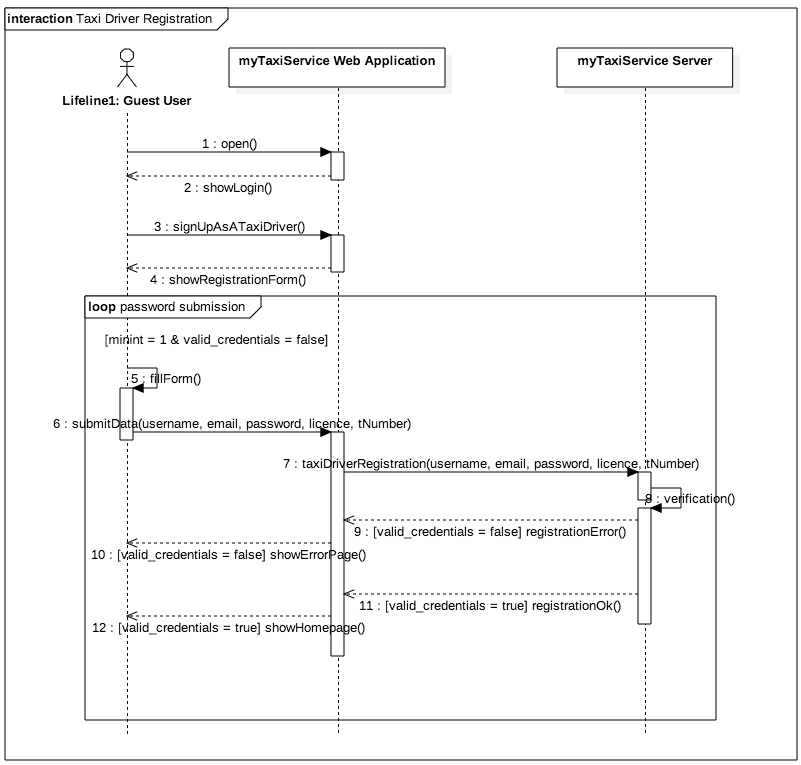
\includegraphics[width=\textwidth, scale=0.5]{IMG/InteractionDiagrams/TaxiDriverRegistration.png}
					\caption{Taxi Driver Registration Interaction Diagram}\label{sec:FigureTaxiDriverRegistration}
				\end{figure}